\section{Présentation}


\begin{frame}
	\begin{center}
		\textbf{Alice \textsc{Dinsenmeyer}}\\
		\footnotesize{Doctorante (1\textsuperscript{ère} année)\\[0.5cm]
		\textit{alice.dinsenmeyer@insa-lyon.fr\\
		1\textsuperscript{er} étage, Bât. J. Jacquard}}
			
	\end{center}
	\begin{itemize}
		\item 2011 -- 2014 : Licence en acoustique, Université du Maine, Le Mans %Bachelor of science in acoustics
		\item 2014 --2016 : Master recherche en acoustique, Université du Maine, Le Mans %Master of science in acoustics
		\begin{columns}
			\hspace{2cm}\column{0.5\textwidth}
			\begin{itemize}
				\item[-] Ondes dans les solides et les fluides
				\item[-] Imagerie ultrasonore
				\item[-] Psychoacoustique
			\end{itemize}
			\column{0.5\textwidth}
			\begin{itemize}
				\item[-] Traitement du signal
				\item[-] Informatique scientifique
			\end{itemize}
		\end{columns}
	\end{itemize}
\end{frame}

\section{Sujet de thèse}


\begin{frame}
	\centering
	\textbf{ Méthodes inverses par approche bayésienne \\pour l'identification de sources aéroacoustique}\\
	\footnotesize{depuis juillet 2017}\\[0.5cm]
	Direction : Jérôme Antoni (LVA), Chritophe Bailly (LMFA), Quentin Leclère (LVA)\\[0.5cm]
	Financements : CeLyA + INSAVALOR (projet européen \textbf{AD}vanced \textbf{A}eroacoustic \textbf{P}rocessing \textbf{T}echniques, ADAPT)

	Collaborations : LVA, LMFA, MicrodB, PSA3, Airbus
\end{frame}


\begin{frame}{Contexte}
	\begin{itemize}
		\item Réduction du bruit des avions (conception et validation) : aérodynamique et turbomachines
		\item Caractériser acoustiquement des flucutations de pressions, dominées par la turbulence
		\item Spécificité des sources aéroacoustique : 
			\begin{itemize}
				\item parcimonieuse spatialement,
				\item large bande fréquentielle (not. domaine de l'audible)
				\item mesures empreintes de bruit aérodynamique
			\end{itemize}
		\item Méthodes actuelles : formation de voies + déconvolution
			\begin{itemize}
				\item Avantages : flexible, simple et rapide
				\item Limites : connaissance du modèle de sources a priori, sources corrélées, artefacts, niveaux
			\end{itemize}
	\end{itemize}
	
\end{frame}


\begin{frame}
	approche bayésienne
\end{frame}

\begin{frame}
	
	Problématiques : \\
	-extraction des composantes tonales, cyclostationnaires et aérodynamiques\\
	-régularisation (prior information)
	-interprétation des résultats
	

	
\end{frame}

\begin{frame}{Imagerie US vs localisation de sources}
	\begin{itemize}
		\item<1-> Localisation de sources acoustique
		\begin{figure}
			
\includegraphics[width = 6cm]{./img/pd_dir_inv/ac.png}
		\end{figure}~\\
		\item<2-> Imagerie par ultrasons
		\begin{figure}
			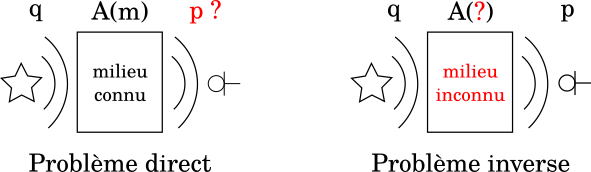
\includegraphics[width = 6cm]{./img/pd_dir_inv/us.png}
		\end{figure}
	\end{itemize}
	
\end{frame}

